% !TEX root = ../paper.tex

%\section{Background}
%In this section, we describe MCR process based on Gerrit system. Then, we describe the background behind our approach composed of text mining techniques using VSM and euclidian distance and prediction evaluation techniques. 
\section{Modern Code Review Process}

An overview of MCR process based on Gerrit system is shown in Figure \ref{fig:process}. The grey area shows the review process of the system which composed of four main steps. (1) an author creating a patch and submitting a set of new or modified files as a review request to Gerrit system. (2) reviewers examine the proposed code changes whether it contains defects or not. (3) reviewers will give comments where should the author improve the code change. The author will create a new change according to the comments then re-submit a new patch again. Then, reviewers will examine the new change. If there is still a needed improvement, reviewers will give comments to fix again. The steps (1)-(3) will be iterated until reviewers can determine that this changes can be merge to the project or should not be merge (reject the change). 

According to this process, reviewers' comment is the most important for the software quality. McIntosh et. al. \cite{Mcintosh} also found that components which were reviewed without discussion are likely to contain bugs. However, as tool supporting MCR allows reviewers freely write a message to the author, it is often seen that some comments are not clearly identify defects and ineffective. Microsoft developers reported that they only focus on minor logic errors rather than discussing deeper in design\cite{Bacchelli2013a}. Our observation in Qt project also correspond this finding. We found some comments are superficial and unrelated to the proposed changes. For example, a superficial and unconfident reviewer as shown in Fig. \ref{fig:example}(a), a comment for rule of using Version Control System (e.g. Git) in the project Fig. \ref{fig:example}(b). 

\begin{figure}[!t]
\centering
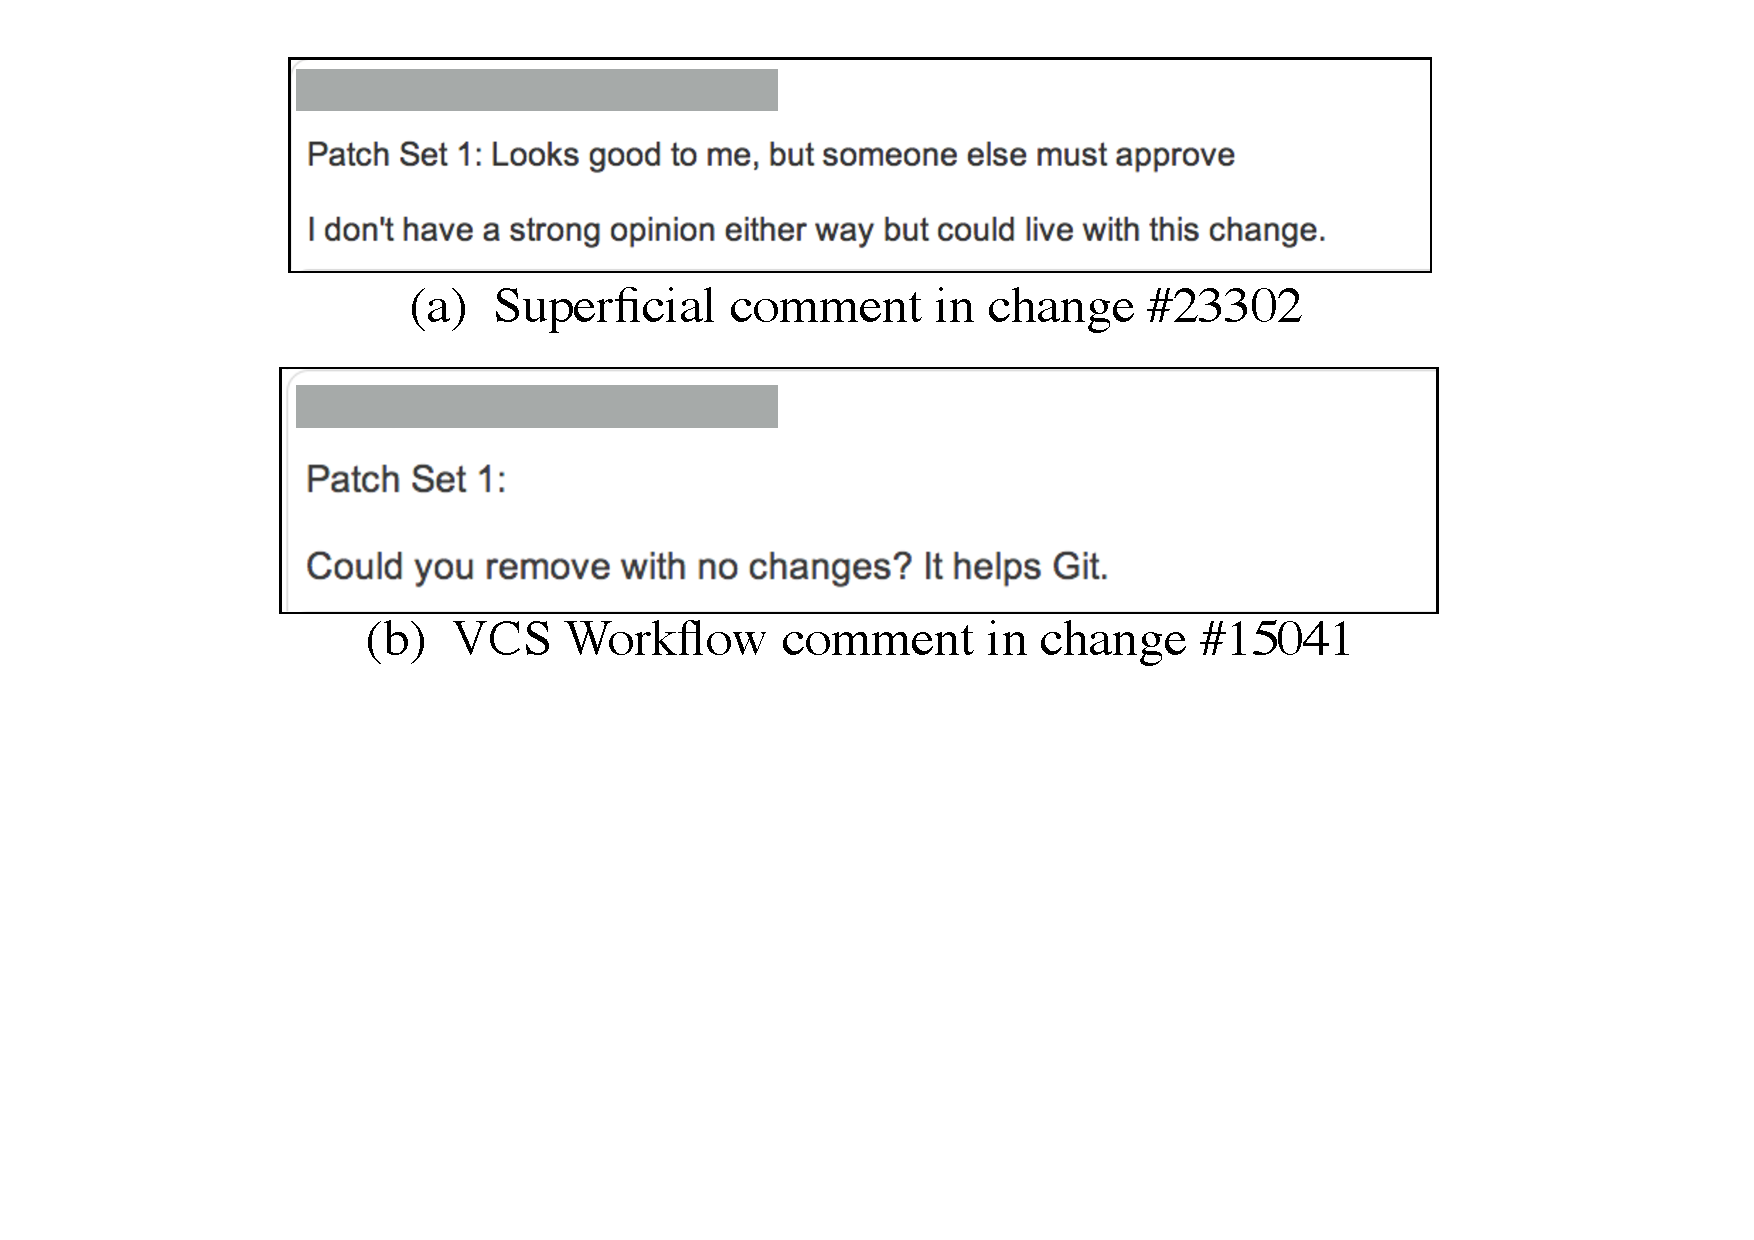
\includegraphics[scale=0.4, trim= 100 250 0 0, clip=true]{comment_examples}
\caption{Examples of comment in code reviews of Qt project.}
\label{fig:example}
\end{figure}




\section{Reviewers' Comments Classification Approach}
\begin{figure}[!t]
\centering
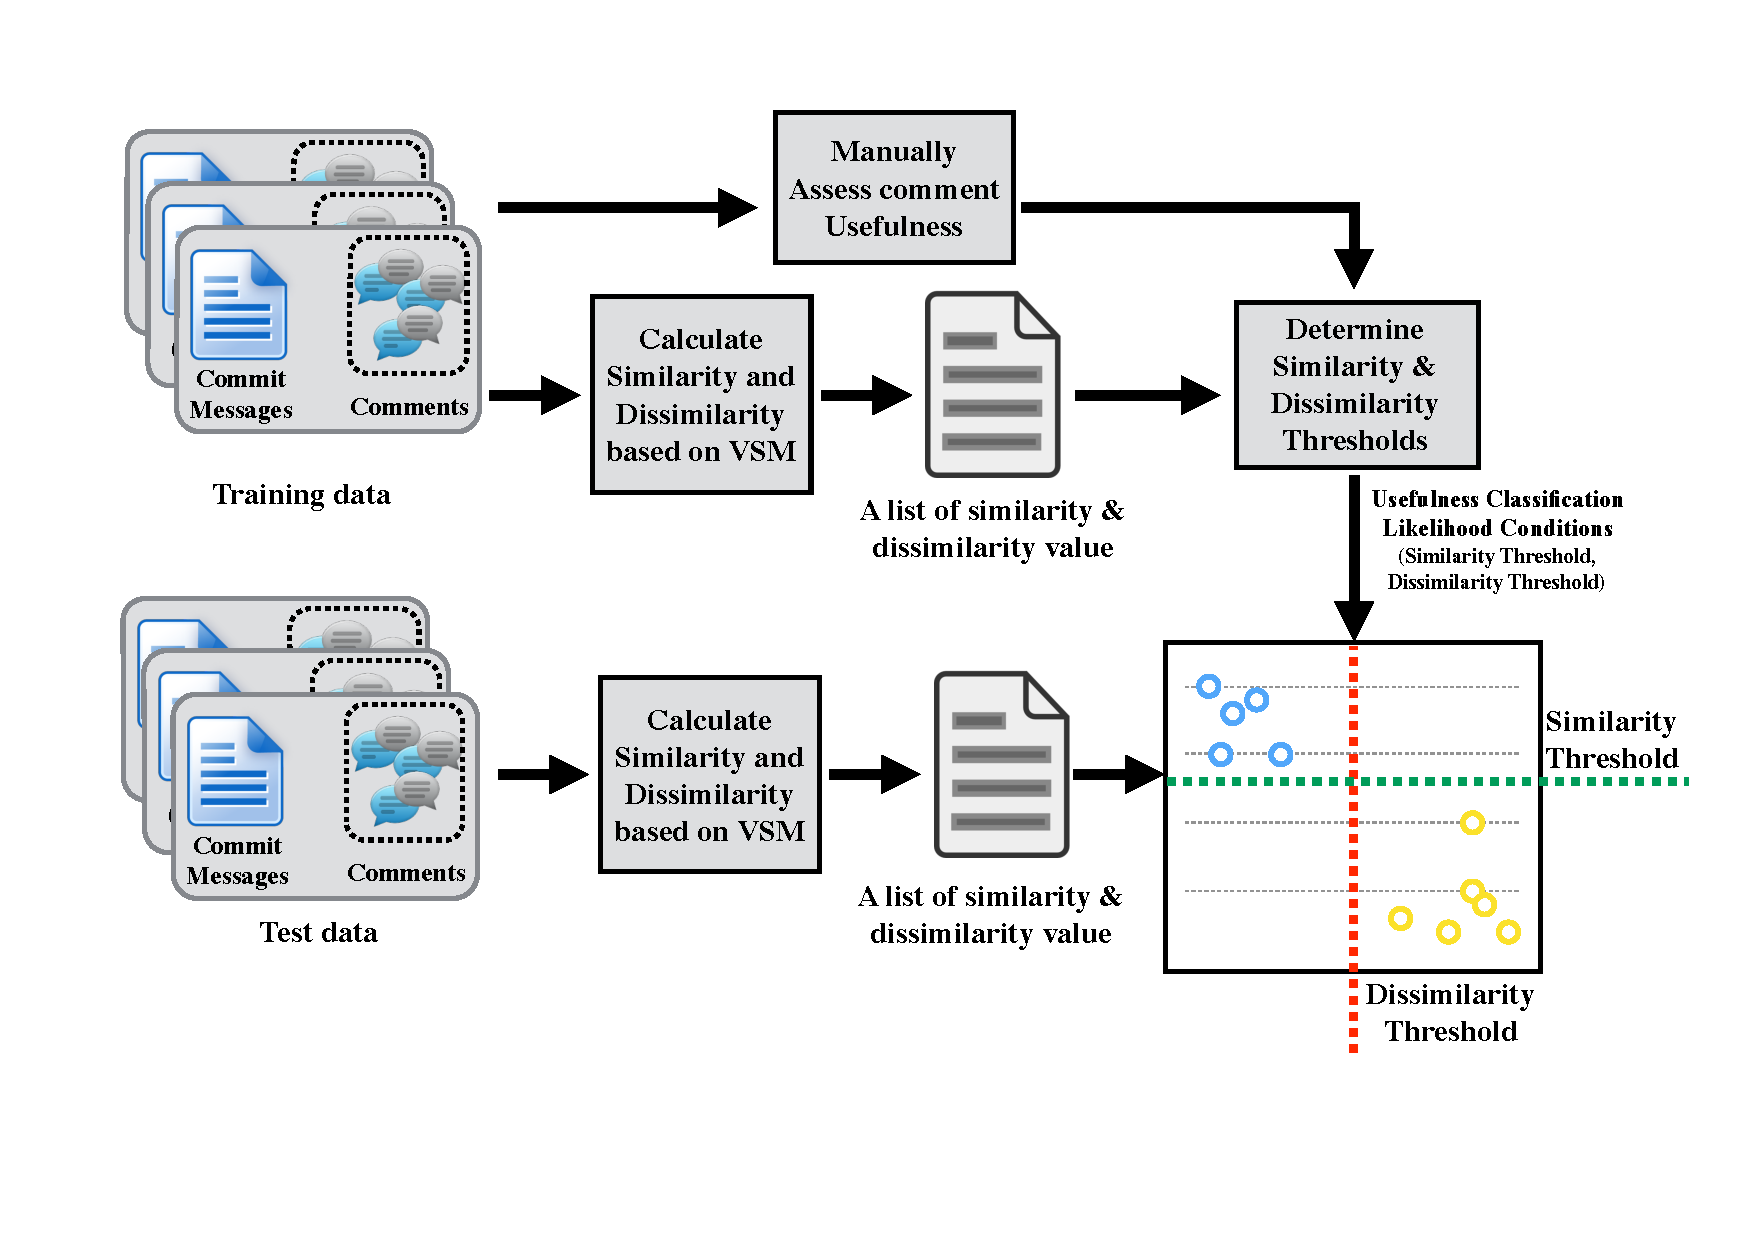
\includegraphics[scale=0.35, trim = 50 90 0 30, clip=true]{overview2}
\caption{Overview of our classification approach.}
\label{fig:overview}
\end{figure}

Figure \ref{fig:overview} shows the overview of our proposed approach. We classify usefulness of comments by measuring similarity between commit message of proposed change and its comments. To calculate similarity in Fig. \ref{fig:overview}(a), we use Vector Space Model (VSM) which is well-known technique for retrieving similar documents written in unstructured natural language. We also use euclidian distance to calculate dissimilarity. For our training dataset, we manually identify every pair of comment and commit messages in Fig. \ref{fig:overview}(b). Then, we use the results from Fig. \ref{fig:overview}(a) and from Fig. \ref{fig:overview}(b) to estimate similarity and dissimilarity threshold that can best discriminate useful/useless comments. Using these thresholds, we can classify the usefulness of comments for the rest of comments in review history. 

To classify usefulness of comment using similarity and dissimilarity, we firstly formalize our classification model as follows:
\begin{itemize}
\item $\Theta(c,S_T,D_T)$ predict as \textbf{useful} if $\mathrm{sim}(m,c) \geq S_T$ and $\mathrm{dist}(m,c) \leq D_T$.
\item $\Omega(c,S'_T,D'_T)$ predict as \textbf{useles} if $\mathrm{sim}(m,c) \leq  S'_T$ and $\mathrm{dist}(m,c) \geq D'_T$.
\end{itemize}
where $S_T$ and $D_T$ are similarity and dissimilarity thresholds for useful comments identification; while $S'_T$ and $D'_T$ are similarity and dissimilarity thresholds for useless comments identification. The functions $\mathrm{sim}(m,c)$ and $\mathrm{dist}(m,c)$ calculates similarity and dissimilarity of comment $c$ comparing with commit message of its review. The details our approach is described in the following subsections.
\pick{Why we need two measurements?}
\pick{What happen in model for otherwise?}

\subsection{Similarity and Dissimilarity Calculation based on VSM}
%Vector Space Model (VSM) is well-known technique for information retrieval where documents written in unstructured natural language. In Software Engineering, VSM has been widely use to find relationship among documents in software issue tracking system\cite{Davies2012}.
For each review, we compute similarity and dissimilarity of every comments comparing with the commit message which is described the purpose of the change.
To do so, we use VSM which is a model for representing text documents as vectors. For a set of commit messages and comments ($D$), each document, $d$ (commit message or comment) is represented as $\overrightarrow{V_d} = <w_{1,d},w_{2,d},w_{3,d},...w_{n,d}>$, where $n$ is the total number of unique terms occur in $D$. The $w_{t,d}$ value is TF-IDF weighting of term $t$ calculated from term occurrence frequency using Equation \ref{eq:tf-idf} where $tf_{t,d}$ is frequency of term $t$ occurs in document $d$; and $|\{d' \in D | t \in d'\}|$ is the number of other documents $d'$ that also contain term $t$.  

\begin{equation}
w_{t,d} = tf_{t,d} \times \log\frac{|D|}{1+|\{d' \in D | t \in d'\}|}
\label{eq:tf-idf}
\end{equation}

After transforming commit message and comments to vectors, we calculate similarity using Cosine similarity and Euclidian distance. 


\noindent\textbf{Cosine similarity} measures similarity between two vectors using inner product. Given a vector commit message $\overrightarrow{V_m}$ and the vector of its comments $\overrightarrow{V_m}$, we can calculate Cosine similarity using Equation \ref{eq:cosine}. The similarity value is ranging $[0,1]$ where 0 means there is no similarity and 1 means two vectors are textually similar.  

\begin{equation}
\mathrm{sim}(m,c) = \cos\theta(\overrightarrow{V_m},\overrightarrow{V_c}) = \frac{\sum_{i=1}^{|D|} w_{i,m} \times w_{i,c}}{\sqrt{\sum_{i=1}^{|D|} w^2_{i,m} \times \sum_{i=1}^{|D|} w^2_{i,c}}}
\label{eq:cosine}
\end{equation}

\noindent\textbf{Euclidian distance} measures ordinary distance between each element of two vectors using Equation \ref{eq:euclid}. We can use this distance as an dissimilarity. Given a vector commit message $\overrightarrow{V_m}$ and the vector of its comments $\overrightarrow{V_m}$, we can calculate Euclidian distance using Equation \ref{eq:cosine}. The distance value is ranging $[0,\infty)$ where 0 means these vectors are the same vectors while a more distance means these vectors are less similar.

\begin{equation}
\mathrm{dist}(m,c) = \mathrm{euclidian}(\overrightarrow{V_m},\overrightarrow{V_c}) = \sqrt{\sum_{i=1}^{|D|}(w_{i,m} - w_{i,c})^2}
\label{eq:euclid}
\end{equation}

\subsection{Estimating Similarity and Dissimilarity Threshold}
We find similarity and dissimilarity thresholds by selecting $s_t,d_t$ values that can maximize $\mathrm{F\text{-}measure}_{s_t,d_t}$. This is an accuracy measurement for a binary classification considering an accuracy of prediction (precision) and  a coverage of classification (recall). This can be calculated using Equation \ref{eq:fmeasure}.

\begin{equation}
\begin{split}
\mathrm{F\text{-}measure}_{s_t,d_t} &= 2 \times \frac{\mathrm{precision}_{s_t,d_t} \times \mathrm{recall}_{s_t,d_t}}{\mathrm{precision}_{s_t,d_t} + \mathrm{recall}_{s_t,d_t}}
\\
\mathrm{precision}_{s_t,d_t}  &= \frac{\mathrm{TP}_{s_t,d_t}}{\mathrm{TP}_{s_t,d_t}+\mathrm{FP}_{s_t,d_t}}
\\
\mathrm{recall}_{s_t,d_t}  &= \frac{\mathrm{TP}_{s_t,d_t}}{\mathrm{TP}_{s_t,d_t}+\mathrm{FN}_{s_t,d_t}}
\end{split}
\label{eq:fmeasure}
\end{equation}




Suppose we use $\Theta(c,S_T=s_t,D_T=d_t)$ as predict model to identify useful comments , $\mathrm{TP}_{s_t,d_t}$ is the number of comments that our model predicted as \textit{useful} and are actually useful; $\mathrm{FP}_{s_t,d_t}$ is the number of comments that our model predicted as \textit{useful} but are actually useless; and $\mathrm{FN}_{\theta_s,\theta_d}$ is the number of comments that our model predict as \textit{useless} but are actually useful. To measuring F-measure for $\Omega(c,S_T=s_t,D_T=d_t)$ model, it uses the same consideration but change the determination to useless comments. For the correctness of prediction, we determine from the useful/useless defined dataset. 


%Using this method, we iteratively measure an accuracy for values of $s_t$ and $s'_t$ ranging $[0,1]$; and values of $d_t$ and $d'_t$ ranging $[0,\infty)$. 

%\begin{equation}
%\mathrm{F\text{-}measure}_{S_T,D_T} = \frac{2\mathrm{TP}_{S_T,D_T}}{2\mathrm{TP}_{S_T,D_T}+\mathrm{FP}_{S_T,D_T}+\mathrm{FN}_{S_T,D_T}}
%\label{eq:precision}
%\end{equation}

%where $\mathrm{TP}_{S_T,D_T}= |\{ c \in C |  \text{\textbf{useful}}(c,S_T,D_T) = \mathrm{TRUE} \}\cap \{c \in C| \mathrm{vote}(c) = 2\}|$,  $\mathrm{FP}_{S_T,D_T} = |\{ c \in C | \text{\textbf{useful}}(c,S_T,D_T) = \mathrm{FALSE} \}\cap \{\mathrm{vote}(c) = 2\} $, $\mathrm{FN}_{S_T,D_T} = |\{ c | c \in C, \text{\textbf{useful}}(c,S_T,D_T) = \mathrm{TRUE} \}\cap \{\mathrm{vote}(c) < 2\} $
%According to this, we can formalize as follows:

%\begin{equation}
%(S_T,D_T) = \max(\{\mathrm{F\text{-}measure} \text{ of \textbf{useful}}(c,s_T,d_T) | s_T\in[0,1] \text{ and } d_T\in [0,\infty) \})
%\end{equation}

